% !TeX root = ../../../金融经济学_王江_讲义及习题.tex
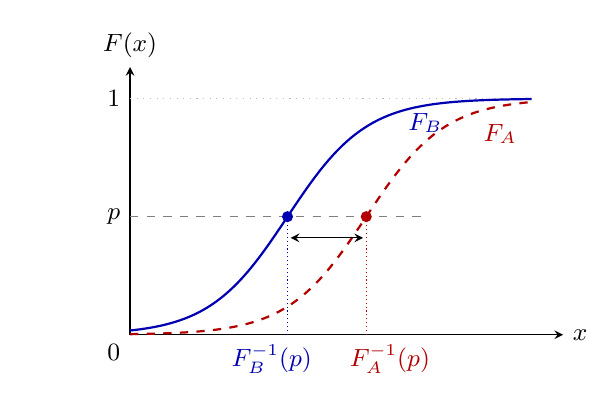
\begin{tikzpicture}[x=1cm,y=1cm,>=stealth,font=\small]
 \path[use as bounding box] (-1.3,-0.65) rectangle (5.8,3.9);
 \draw[->] (0,0)--(5.5,0) node[right] {$x$};
 \draw[->] (0,0)--(0,3.4) node[above] {$F(x)$};
 \node[below left] at (0,0) {$0$};
 \draw[gray!55,dotted] (0,3)--(5.1,3);
 \node[left] at (0,3) {$1$};
 \draw[blue!70!black,thick,domain=0:5.1,samples=90]
   plot (\x,{3/(1+exp(-2*(\x-2)))});
 \draw[red!70!black,thick,dashed,domain=0:5.1,samples=90]
   plot (\x,{3/(1+exp(-2*(\x-3)))});
 \node[blue!70!black,below] at (3.75,2.94) {$F_B$};
 \node[red!70!black,below] at (4.7,2.8) {$F_A$};
 \draw[gray,dashed] (0,1.5)--(3.7,1.5);
 \node[left] at (0,1.5) {$p$};
 \draw[blue!70!black,densely dotted] (2,0)--(2,1.5);
 \draw[red!70!black,densely dotted] (3,0)--(3,1.5);
 \fill[blue!70!black] (2,1.5) circle (2pt);
 \fill[red!70!black] (3,1.5) circle (2pt);
 \node[below,blue!70!black] at (1.8,0) {$F_B^{-1}(p)$};
 \node[below,red!70!black] at (3.3,0) {$F_A^{-1}(p)$};
 \draw[<->] (2.04,1.23)--(2.96,1.23);
\end{tikzpicture}%
